
%(BEGIN_QUESTION)
% Copyright 2009, Tony R. Kuphaldt, released under the Creative Commons Attribution License (v 1.0)
% This means you may do almost anything with this work of mine, so long as you give me proper credit

Connect a ``smart'' (HART protocol) loop-powered to a DC voltage source, a 250 ohm resistor, and a diode as shown, using parts supplied by the instructor.  All electrical connections must be made using a terminal strip (no twisted wires, crimp splices, wire nuts, spring clips, or ``alligator'' clips permitted):

$$\includegraphics[width=15.5cm]{i03878x01.eps}$$

\vskip 10pt

After building your circuit, answer the following questions:

\begin{itemize}
\item{} Connect a HART communicator device in parallel with the transmitter, turn it on, and use it to access the transmitter's programmable parameters.
\vskip 10pt
\item{} Use a multimeter set to measure {\it AC} volts to detect HART communications in the circuit.  What happens to the AC voltage measurement when the HART communicator is turned off?  Is there any way to capture the peak HART signal values using your multimeter?
\vskip 10pt
\item{} Temporarily short past the resistor with a jumper wire and note whether or not this has any effect on the 4-20 mA analog current signal.  Also note whether this elimination of the resistor has any effect on the ability of the transmitter to communicate using HART (digital) signals.
\end{itemize}

\vskip 20pt \vbox{\hrule \hbox{\strut \vrule{} {\bf Suggestions for Socratic discussion} \vrule} \hrule}

\begin{itemize}
\item{} It is possible to properly connect a HART communicator to a HART instrument and still not have it ``talk.''  The communicator must also be programmed with a {\it Device Description} (DD) for the HART instrument in order to communicate and access all its parameters.  Explain they purpose and rationale for Device Descriptions.
\end{itemize}

\underbar{file i03878}
%(END_QUESTION)





%(BEGIN_ANSWER)


%(END_ANSWER)





%(BEGIN_NOTES)

$$\includegraphics[width=15.5cm]{i03878x01.eps}$$

\vskip 20pt \vbox{\hrule \hbox{\strut \vrule{} {\bf Virtual Troubleshooting} \vrule} \hrule}

This question is a good candidate for a ``Virtual Troubleshooting'' exercise.  Presenting the diagram to students, you first imagine in your own mind a particular fault in the system.  Then, you present one or more symptoms of that fault (something noticeable by an operator or other user of the system).  Students then propose various diagnostic tests to perform on this system to identify the nature and location of the fault, as though they were technicians trying to troubleshoot the problem.  Your job is to tell them what the result(s) would be for each of the proposed diagnostic tests, documenting those results where all the students can see.

During and after the exercise, it is good to ask students follow-up questions such as:

\begin{itemize}
\item{} What does the result of the last diagnostic test tell you about the fault?
\item{} Suppose the results of the last diagnostic test were different.  What then would that result tell you about the fault?
\item{} Is the last diagnostic test the best one we could do?
\item{} What would be the ideal order of tests, to diagnose the problem in as few steps as possible?
\end{itemize}

%INDEX% Fieldbus, HART: transmitter circuit

%(END_NOTES)





